\documentclass[a4paper, 12pt]{article}
\usepackage{graphicx} % Required for inserting images
\usepackage{fullpage}
\usepackage{amsmath}
\usepackage{xcolor}
\usepackage{float}
\usepackage{geometry}
\usepackage{biblatex}
\geometry{margin=1in}
\usepackage{enumitem}
\usepackage{hyperref}
\usepackage{parskip}
\usepackage[version=4]{mhchem}
\title{Chemistry Honors Study Guide}
\author{Test 1 S1}
\date{Test date: September 25, 2024}

\begin{document}

\maketitle

\begin{center}
    (All links are clickable!)
\end{center}

\section{Basic Scientific Concepts}

\subsection*{Definitions}

\begin{itemize}[leftmargin=*, nosep]
    \item \textbf{\textit{scientific law:}} A statement describing or predicting natural phenomena.
    \item \textbf{\textit{scientific theory:}} An explanation for natural phenomena.
    \item \textbf{\textit{accuracy:}} A measure of how close measurements are to the true value.
    \item \textbf{\textit{precision:}} A measure of how close measurements are to each other.
    \item \textbf{\textit{physical property:}} A characteristic of a substance that can be observed or measured without altering its identity.
    \item \textbf{\textit{chemical property:}} A characteristic of a substance that can only be observed or measured when a chemical reaction occurs (the substance is converted into a different substance). 
\end{itemize}

\subsection*{The Scientific Method}
make an \textbf{observation} $\xrightarrow{}$ ask a \textbf{question} $\xrightarrow{}$ background \textbf{research} $\xrightarrow{}$ form a \textbf{hypothesis} $\xrightarrow{}$ \textbf{test} the hypothesis $\xrightarrow{}$ \textbf{analyze} the data $\xrightarrow{}$ \textbf{communicate} your findings... and repeat!

\subsection*{Law v. Theory}
\textbf{Law} is the \textbf{``what"}, while \textbf{theory} is the \textbf{``why"}. Both have been proven but can be disproven and are supported by scientific consensus.  
 
Example: Newton's First Law, also known as the \textcolor{blue}{law of inertia}, states that an object at rest will remain at rest unless acted upon by an outside force. This is an example of a law because it simply explains what happens (i.e. it is predictive). On the other hand, the theory of \textcolor{blue}{evolution by natural selection} is classified as theory because it is a comprehensive explanation based on an observation.

\subsection*{Accuracy v. Precision}
Having both accuracy and precision (see definitions above) is ideal for data collection. Here are some examples of one, both, or neither (where true value = 1.0):
 
\textbf{Accurate, but not precise:} 1.17, 1.28, 0.85
\\
\textbf{Precise, but not accurate:} 2.8, 2.75, 2.9
\\
\textbf{Accurate and precise:} 1.1, 1.0, 1.01
\\
\textbf{Neither accurate nor precise:} 6.08, 3.1, 0.5


\subsection*{Physical v. Chemical Properties}
(\underline{not an exhaustive list})

\subsubsection*{Physical Properties}
\begin{itemize}[leftmargin=*, nosep]
    \item Color
    \item Melting/Boiling point
    \item Density
    \item Solubility
    \item Conductivity
\end{itemize}

\subsubsection*{Chemical Properties}
\begin{itemize}[leftmargin=*, nosep]
    \item Reactivity
    \item Smell
    \item Flammability
    \item Toxicity
    \item pH
\end{itemize}

\subsection*{Classifying Matter}

\subsubsection*{Classifying By Phase}
\textbf{Solid:} holds its shape, not compressible, closely packed, fixed relative positions.
\\
\textbf{Liquid:} conforms to container, not compressible, unfixed relative positions, closely packed.
\\
\textbf{Gas:} conforms to container, compressible, unfixed relative positions, loosely packed.
\\
\textbf{Plasma:} an ionized gas with electrical charge. 

\subsubsection*{Classifying By Composition}
\underline{Matter}: \textbf{pure substance} or \textbf{mixture}
\\
\underline{Pure substance:} \textbf{element} \textcolor{blue}{(Au, Ag, Fe, Pb, S$_8$)} or \textbf{compound} \textcolor{blue}{(H$_2$O, NaCO$_3$, CO$_2$, C$_6$H$_{\text{12}}$O$_6$)}
\\
\underline{mixture:} \textbf{homogeneous}, uniformly mixed \textcolor{blue}{(solutions, alloys, dish soap)} or \textbf{heterogeneous}, not uniformly mixed \textcolor{blue}{(oil + water, sand + salt, salad, milk)}

\section{Basic Mathematical Concepts}

\subsection*{Significant Digits}
\textbf{Rules for Significant Digits:}
\begin{enumerate}[leftmargin=*, nosep]
    \item All nonzero digits are significant.
    \item Leading zeros (to the left of the first nonzero digit) are never significant.
    \item Trailing zeros are only significant if there is a decimal point.
    \item All zeros between nonzero digits are significant.
\end{enumerate}

\subsection*{Scientific Notation}
$$3.14 \times 10^3$$
\\
The first number must be \textbf{$\geq$1} and \textbf{$\leq$10}. When changing a number from scientific notation to standard form (or vice versa), \textbf{the number of significant figures stays the same.}

\subsection*{Metric Units}
\begin{center}
\begin{tabular}{c|c|c}
   \textbf{Prefix} & \textbf{Abbreviation} & \textbf{Value} \\\hline
    kilo- & k & 10$^3$ \\
    centi- & c & 10$^{\text{-2}}$ \\
    milli- & m & 10$^{\text{-3}}$ \\
    micro- & $\mu$ & 10$^{\text{-6}}$ \\
    nano- & n & 10$^{\text{-9}}$ \\
\end{tabular}
\end{center}

\subsubsection*{Metric Unit Conversions}
Question: How many micrometers are in 456 kilometers? (1 kilometer = 1,000,000,000 micrometers)

$$456 \: km \times \frac{1,000,000,000 \: \mu m}{1 \: km} = 456,000,000,000 \: \mu m$$
\\
\noindent The first number is the number of kilometers there were in the original question; the second is the unit fraction (equal to 1). The original unit ($km$, in this case) should be put at the bottom of the fraction so it cancels out.

\section{The Periodic Table of Elements}

\textcolor{teal}{{\href{https://ptable.com}{Online Periodic Table}}}

\subsection*{Definitions}
\begin{itemize}[leftmargin=*, nosep]
    \item \textbf{\textit{Aufbau principle:}} States that electrons first occupy the orbitals with the lowest energy.
    \item \textbf{\textit{isotopes:}} Atoms of the same element (same number of protons) with different atomic masses (different number of neutrons).
    \item \textbf{\textit{Pauli exclusion principle:}} States that no two electrons in the same atom can have the same four quantum numbers.
\end{itemize}

\subsection*{Classifications}

\begin{itemize}[leftmargin=*, nosep]
    \item Group 1: \textbf{alkali metals}
    \item Group 2: \textbf{alkali earth metals}
    \item Groups 3-12: \textbf{transition metals}
    \item Group 17: \textbf{halogens}
    \item Group 18: \textbf{noble gases}
\end{itemize}

\subsection*{Properties}
\textbf{Metals} are \textbf{good conductors of heat and electricity}, \textbf{malleable}, \textbf{ductile}, and \textbf{shiny}.
\\
\textbf{Nonmetals} are \textbf{insulators} (not conductive) and \textbf{brittle.}
\\
\textbf{Metalloids}, also known as semi-conductors, are \textbf{semi-conductive}.

\subsection*{The Atom\footnote{www.universetoday.com/56469/atom-diagram/\#google\_vignette}}

\begin{center}
\begin{tabular}{c|c|c|c}

     \textbf{Name} & \textbf{Mass (amu)} & \textbf{Charge} & \textbf{Location} \\\hline
     proton & 1 & +1 & nucleus \\
     neutron & 1 & 0 & nucleus \\
     electron & negligible & -1 & orbitals
\end{tabular}
\end{center}

\begin{figure}[ht]
    \centering
    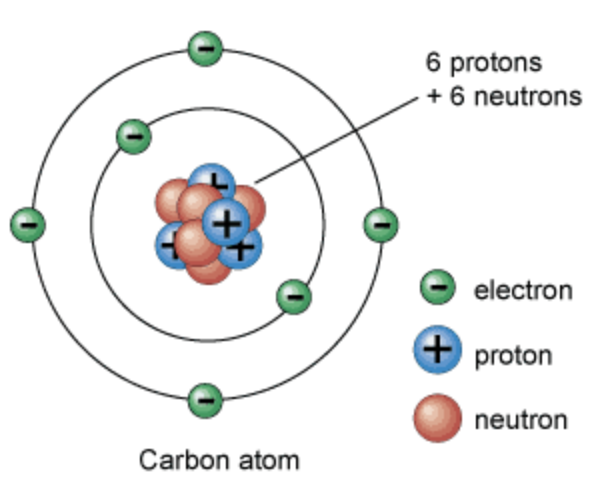
\includegraphics[width=0.5\linewidth]{atom.png}
    \label{fig:1}
\end{figure}

\subsection*{Electron Configuration}
\subsubsection*{Full Electron Configuration\footnote{https://madoverchemistry.com/2017/03/14/41-the-periodic-table-spdf-blocks/}}
Electrons can exist in 4 types of orbitals: s, p, d, and f. \textbf{s, p, and d} are the only orbitals that will appear on the test. Each orbital can hold a maximum of \textbf{2 electrons.}

\begin{figure}[H]
    \centering
    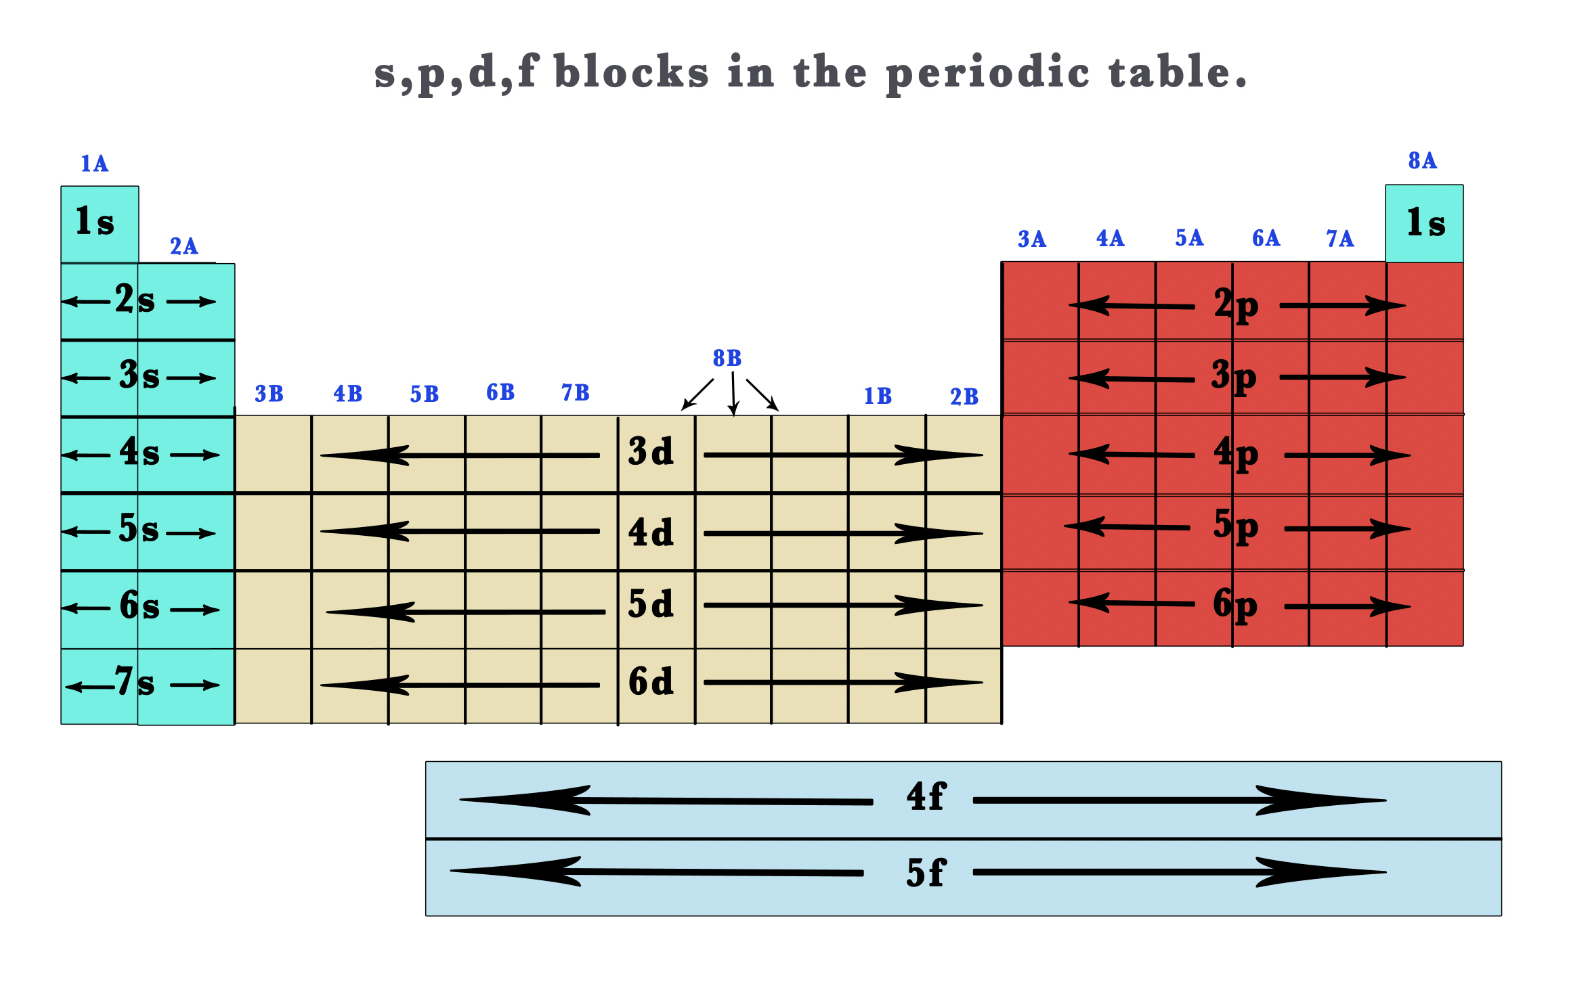
\includegraphics[width=0.7\linewidth]{spdfblocks.png}
    \label{fig:2}
\end{figure}
\noindent There is/are \textbf{1 $s$ orbital}, \textbf{3 $p$ orbitals}, and \textbf{5 $d$ orbitals\footnote{$d$ orbitals appear only after 4$s$.}} per energy level. More energy levels are added with more rows on the periodic table. The electron configuration is a notation that specifies the energy level, the type of orbital, and the number of electrons in that specific orbital. According to the Aufbau Principle, orbitals are filled in this order: 

\begin{figure}[H]
    \centering
    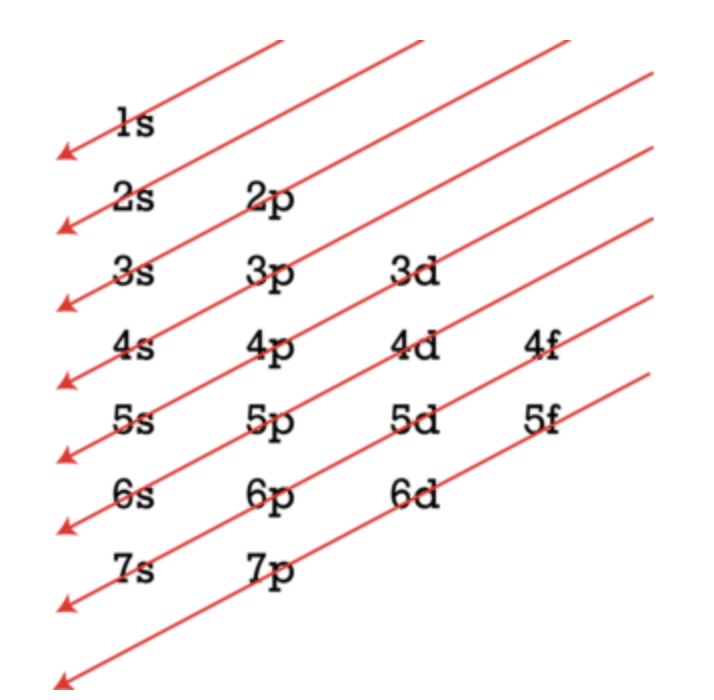
\includegraphics[width=0.4\linewidth]{aufbauprinciple.png}
    \label{fig:3}
\end{figure}

\noindent In the following example, the superscript indicates the number of electrons, the letter indicates the orbital type, and the number indicates the energy level.
 
Example: \textcolor{blue}{Bromine (Br): $1s^22s^22p^63s^23p^5$}

\subsubsection*{Noble Gas Configuration}
For noble gas configurations, take the name of the last noble gas, put it in brackets, then write the rest of the configuration, omitting that of the noble gas.
 
Example: \textcolor{blue}{Bromine (Br): $[Ne]3s^23p^5$}

\subsection*{Electron Box Diagrams}
In electron box diagrams, each box represents an orbital. (The boxes will already be drawn on the test.)
\subsubsection*{Things to remember:}
\begin{itemize}[leftmargin=*, nosep]
    \item Two arrows in the same box should be pointing in different directions (one up, one down).
    \item For multiple orbitals, place an arrow in each orbital first.
\end{itemize}

\begin{figure}[ht]
    \centering
    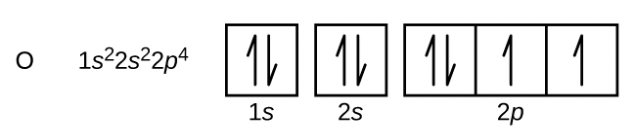
\includegraphics[width=0.5\linewidth]{electronboxdiagrams.png}
    \label{fig:4}
\end{figure}

\subsection*{Ions}
The charge on particles is determined by adding the number of negative charges (adding a negative number) to the number of positive charges.
 
Example: The charge on an element with 5 protons and 2 electrons is \textcolor{blue}{+3}.

\subsection*{Isotopic Symbols}
\ce{^{A}_{B}X} or \ce{^{A}X} or X-A
 
where:
\begin{itemize}[leftmargin=*, nosep]
    \item X = atomic symbol
    \item A = mass number (protons + neutrons)
    \item B = atomic number
\end{itemize}

\subsection*{Quantum Numbers}

\textbf{$n$}, the \textbf{principle quantum number,} indicates the \textbf{orbital shell} in which an electron is in (1, 2, 3, 4, etc.)
 
\textbf{$l$}, the \textbf{angular quantum number,} indicates the \textbf{orbital type.}
\\
$s$ orbital $\xrightarrow{}$ 0
\\
$p$ orbital $\xrightarrow{}$ 1
\\
$d$ orbital $\xrightarrow{}$ 2
 
\textbf{$m_l$}, the \textbf{magnetic quantum number,} indicates the specific orbital in which the electron is located. The number of possibilities for $m_l$ correspond to the number of orbitals.
\\
$s$ orbital $\xrightarrow{}$ 0
\\
$p$ orbital $\xrightarrow{}$ -1, 0, 1
\\
$d$ orbital $\xrightarrow{}$ -2, -1, 0, 1, 2
 
\textbf{$m_s$}, the \textbf{spin quantum number,} indicates the spin on the electron. Electrons in the same orbital have opposite spins. The only two possibilities for this number are +$\frac{1}{2}$ and -$\frac{1}{2}$.


\end{document}
